% Created by tikzDevice version 0.12 on 2019-06-13 13:45:03
% !TEX encoding = UTF-8 Unicode
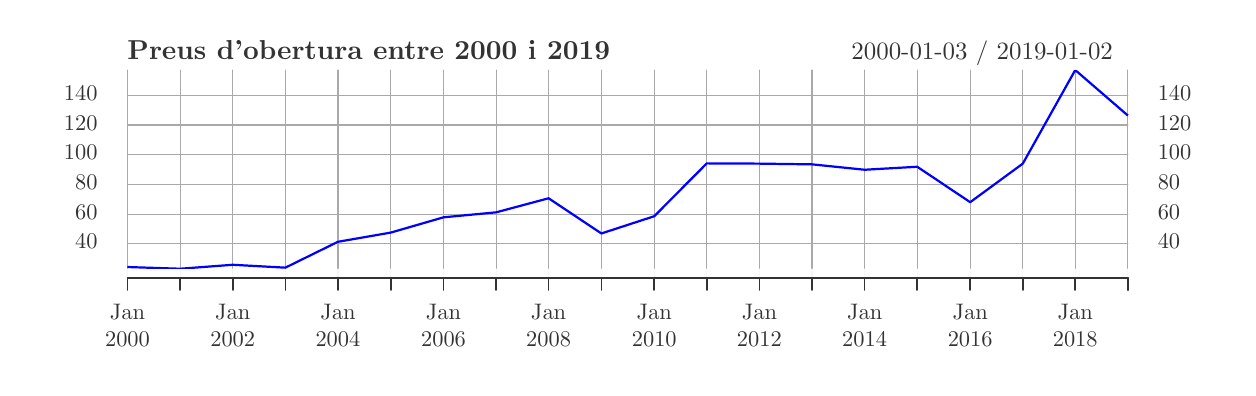
\begin{tikzpicture}[x=1pt,y=1pt]
\definecolor{fillColor}{RGB}{255,255,255}
\path[use as bounding box,fill=fillColor,fill opacity=0.00] (0,0) rectangle (433.62,122.86);
\begin{scope}
\path[clip] ( 21.60, 32.40) rectangle (412.02,122.86);
\definecolor{drawColor}{RGB}{169,169,169}

\path[draw=drawColor,line width= 0.4pt,line join=round,line cap=round] ( 36.06, 35.75) -- ( 36.06,107.54);

\path[draw=drawColor,line width= 0.4pt,line join=round,line cap=round] ( 55.08, 35.75) -- ( 55.08,107.54);

\path[draw=drawColor,line width= 0.4pt,line join=round,line cap=round] ( 74.09, 35.75) -- ( 74.09,107.54);

\path[draw=drawColor,line width= 0.4pt,line join=round,line cap=round] ( 93.11, 35.75) -- ( 93.11,107.54);

\path[draw=drawColor,line width= 0.4pt,line join=round,line cap=round] (112.12, 35.75) -- (112.12,107.54);

\path[draw=drawColor,line width= 0.4pt,line join=round,line cap=round] (131.24, 35.75) -- (131.24,107.54);

\path[draw=drawColor,line width= 0.4pt,line join=round,line cap=round] (150.26, 35.75) -- (150.26,107.54);

\path[draw=drawColor,line width= 0.4pt,line join=round,line cap=round] (169.27, 35.75) -- (169.27,107.54);

\path[draw=drawColor,line width= 0.4pt,line join=round,line cap=round] (188.23, 35.75) -- (188.23,107.54);

\path[draw=drawColor,line width= 0.4pt,line join=round,line cap=round] (207.30, 35.75) -- (207.30,107.54);

\path[draw=drawColor,line width= 0.4pt,line join=round,line cap=round] (226.42, 35.75) -- (226.42,107.54);

\path[draw=drawColor,line width= 0.4pt,line join=round,line cap=round] (245.39, 35.75) -- (245.39,107.54);

\path[draw=drawColor,line width= 0.4pt,line join=round,line cap=round] (264.40, 35.75) -- (264.40,107.54);

\path[draw=drawColor,line width= 0.4pt,line join=round,line cap=round] (283.42, 35.75) -- (283.42,107.54);

\path[draw=drawColor,line width= 0.4pt,line join=round,line cap=round] (302.43, 35.75) -- (302.43,107.54);

\path[draw=drawColor,line width= 0.4pt,line join=round,line cap=round] (321.45, 35.75) -- (321.45,107.54);

\path[draw=drawColor,line width= 0.4pt,line join=round,line cap=round] (340.57, 35.75) -- (340.57,107.54);

\path[draw=drawColor,line width= 0.4pt,line join=round,line cap=round] (359.58, 35.75) -- (359.58,107.54);

\path[draw=drawColor,line width= 0.4pt,line join=round,line cap=round] (378.54, 35.75) -- (378.54,107.54);

\path[draw=drawColor,line width= 0.4pt,line join=round,line cap=round] (397.56, 35.75) -- (397.56,107.54);

\path[draw=drawColor,line width= 0.4pt,line join=round,line cap=round] (397.56, 35.75) -- (397.56,107.54);
\end{scope}
\begin{scope}
\path[clip] (  0.00,  0.00) rectangle (433.62,122.86);
\definecolor{drawColor}{gray}{0.96}

\path[draw=drawColor,line width= 0.4pt,line join=round,line cap=round] ( 36.06, 32.40) -- (397.56, 32.40);

\path[draw=drawColor,line width= 0.4pt,line join=round,line cap=round] ( 36.06, 32.40) -- ( 36.06, 35.64);

\path[draw=drawColor,line width= 0.4pt,line join=round,line cap=round] ( 55.08, 32.40) -- ( 55.08, 35.64);

\path[draw=drawColor,line width= 0.4pt,line join=round,line cap=round] ( 74.09, 32.40) -- ( 74.09, 35.64);

\path[draw=drawColor,line width= 0.4pt,line join=round,line cap=round] ( 93.11, 32.40) -- ( 93.11, 35.64);

\path[draw=drawColor,line width= 0.4pt,line join=round,line cap=round] (112.12, 32.40) -- (112.12, 35.64);

\path[draw=drawColor,line width= 0.4pt,line join=round,line cap=round] (131.24, 32.40) -- (131.24, 35.64);

\path[draw=drawColor,line width= 0.4pt,line join=round,line cap=round] (150.26, 32.40) -- (150.26, 35.64);

\path[draw=drawColor,line width= 0.4pt,line join=round,line cap=round] (169.27, 32.40) -- (169.27, 35.64);

\path[draw=drawColor,line width= 0.4pt,line join=round,line cap=round] (188.23, 32.40) -- (188.23, 35.64);

\path[draw=drawColor,line width= 0.4pt,line join=round,line cap=round] (207.30, 32.40) -- (207.30, 35.64);

\path[draw=drawColor,line width= 0.4pt,line join=round,line cap=round] (226.42, 32.40) -- (226.42, 35.64);

\path[draw=drawColor,line width= 0.4pt,line join=round,line cap=round] (245.39, 32.40) -- (245.39, 35.64);

\path[draw=drawColor,line width= 0.4pt,line join=round,line cap=round] (264.40, 32.40) -- (264.40, 35.64);

\path[draw=drawColor,line width= 0.4pt,line join=round,line cap=round] (283.42, 32.40) -- (283.42, 35.64);

\path[draw=drawColor,line width= 0.4pt,line join=round,line cap=round] (302.43, 32.40) -- (302.43, 35.64);

\path[draw=drawColor,line width= 0.4pt,line join=round,line cap=round] (321.45, 32.40) -- (321.45, 35.64);

\path[draw=drawColor,line width= 0.4pt,line join=round,line cap=round] (340.57, 32.40) -- (340.57, 35.64);

\path[draw=drawColor,line width= 0.4pt,line join=round,line cap=round] (359.58, 32.40) -- (359.58, 35.64);

\path[draw=drawColor,line width= 0.4pt,line join=round,line cap=round] (378.54, 32.40) -- (378.54, 35.64);

\path[draw=drawColor,line width= 0.4pt,line join=round,line cap=round] (397.56, 32.40) -- (397.56, 35.64);
\end{scope}
\begin{scope}
\path[clip] (  0.00,  0.00) rectangle (433.62,122.86);
\definecolor{drawColor}{gray}{0.20}

\path[draw=drawColor,line width= 0.4pt,line join=round,line cap=round] ( 36.06, 32.40) -- (397.56, 32.40);

\path[draw=drawColor,line width= 0.6pt,line join=round,line cap=round] ( 36.06, 32.40) -- ( 36.06, 28.08);

\path[draw=drawColor,line width= 0.6pt,line join=round,line cap=round] ( 55.08, 32.40) -- ( 55.08, 28.08);

\path[draw=drawColor,line width= 0.6pt,line join=round,line cap=round] ( 74.09, 32.40) -- ( 74.09, 28.08);

\path[draw=drawColor,line width= 0.6pt,line join=round,line cap=round] ( 93.11, 32.40) -- ( 93.11, 28.08);

\path[draw=drawColor,line width= 0.6pt,line join=round,line cap=round] (112.12, 32.40) -- (112.12, 28.08);

\path[draw=drawColor,line width= 0.6pt,line join=round,line cap=round] (131.24, 32.40) -- (131.24, 28.08);

\path[draw=drawColor,line width= 0.6pt,line join=round,line cap=round] (150.26, 32.40) -- (150.26, 28.08);

\path[draw=drawColor,line width= 0.6pt,line join=round,line cap=round] (169.27, 32.40) -- (169.27, 28.08);

\path[draw=drawColor,line width= 0.6pt,line join=round,line cap=round] (188.23, 32.40) -- (188.23, 28.08);

\path[draw=drawColor,line width= 0.6pt,line join=round,line cap=round] (207.30, 32.40) -- (207.30, 28.08);

\path[draw=drawColor,line width= 0.6pt,line join=round,line cap=round] (226.42, 32.40) -- (226.42, 28.08);

\path[draw=drawColor,line width= 0.6pt,line join=round,line cap=round] (245.39, 32.40) -- (245.39, 28.08);

\path[draw=drawColor,line width= 0.6pt,line join=round,line cap=round] (264.40, 32.40) -- (264.40, 28.08);

\path[draw=drawColor,line width= 0.6pt,line join=round,line cap=round] (283.42, 32.40) -- (283.42, 28.08);

\path[draw=drawColor,line width= 0.6pt,line join=round,line cap=round] (302.43, 32.40) -- (302.43, 28.08);

\path[draw=drawColor,line width= 0.6pt,line join=round,line cap=round] (321.45, 32.40) -- (321.45, 28.08);

\path[draw=drawColor,line width= 0.6pt,line join=round,line cap=round] (340.57, 32.40) -- (340.57, 28.08);

\path[draw=drawColor,line width= 0.6pt,line join=round,line cap=round] (359.58, 32.40) -- (359.58, 28.08);

\path[draw=drawColor,line width= 0.6pt,line join=round,line cap=round] (378.54, 32.40) -- (378.54, 28.08);

\path[draw=drawColor,line width= 0.6pt,line join=round,line cap=round] (397.56, 32.40) -- (397.56, 28.08);

\path[draw=drawColor,line width= 0.6pt,line join=round,line cap=round] (397.56, 32.40) -- (397.56, 28.08);

\node[text=drawColor,anchor=base,inner sep=0pt, outer sep=0pt, scale=  0.81] at ( 36.06, 27.00) {};

\node[text=drawColor,anchor=base,inner sep=0pt, outer sep=0pt, scale=  0.81] at ( 36.06, 17.28) {Jan};

\node[text=drawColor,anchor=base,inner sep=0pt, outer sep=0pt, scale=  0.81] at ( 36.06,  7.56) {2000};

\node[text=drawColor,anchor=base,inner sep=0pt, outer sep=0pt, scale=  0.81] at ( 74.09, 27.00) {};

\node[text=drawColor,anchor=base,inner sep=0pt, outer sep=0pt, scale=  0.81] at ( 74.09, 17.28) {Jan};

\node[text=drawColor,anchor=base,inner sep=0pt, outer sep=0pt, scale=  0.81] at ( 74.09,  7.56) {2002};

\node[text=drawColor,anchor=base,inner sep=0pt, outer sep=0pt, scale=  0.81] at (112.12, 27.00) {};

\node[text=drawColor,anchor=base,inner sep=0pt, outer sep=0pt, scale=  0.81] at (112.12, 17.28) {Jan};

\node[text=drawColor,anchor=base,inner sep=0pt, outer sep=0pt, scale=  0.81] at (112.12,  7.56) {2004};

\node[text=drawColor,anchor=base,inner sep=0pt, outer sep=0pt, scale=  0.81] at (150.26, 27.00) {};

\node[text=drawColor,anchor=base,inner sep=0pt, outer sep=0pt, scale=  0.81] at (150.26, 17.28) {Jan};

\node[text=drawColor,anchor=base,inner sep=0pt, outer sep=0pt, scale=  0.81] at (150.26,  7.56) {2006};

\node[text=drawColor,anchor=base,inner sep=0pt, outer sep=0pt, scale=  0.81] at (188.23, 27.00) {};

\node[text=drawColor,anchor=base,inner sep=0pt, outer sep=0pt, scale=  0.81] at (188.23, 17.28) {Jan};

\node[text=drawColor,anchor=base,inner sep=0pt, outer sep=0pt, scale=  0.81] at (188.23,  7.56) {2008};

\node[text=drawColor,anchor=base,inner sep=0pt, outer sep=0pt, scale=  0.81] at (226.42, 27.00) {};

\node[text=drawColor,anchor=base,inner sep=0pt, outer sep=0pt, scale=  0.81] at (226.42, 17.28) {Jan};

\node[text=drawColor,anchor=base,inner sep=0pt, outer sep=0pt, scale=  0.81] at (226.42,  7.56) {2010};

\node[text=drawColor,anchor=base,inner sep=0pt, outer sep=0pt, scale=  0.81] at (264.40, 27.00) {};

\node[text=drawColor,anchor=base,inner sep=0pt, outer sep=0pt, scale=  0.81] at (264.40, 17.28) {Jan};

\node[text=drawColor,anchor=base,inner sep=0pt, outer sep=0pt, scale=  0.81] at (264.40,  7.56) {2012};

\node[text=drawColor,anchor=base,inner sep=0pt, outer sep=0pt, scale=  0.81] at (302.43, 27.00) {};

\node[text=drawColor,anchor=base,inner sep=0pt, outer sep=0pt, scale=  0.81] at (302.43, 17.28) {Jan};

\node[text=drawColor,anchor=base,inner sep=0pt, outer sep=0pt, scale=  0.81] at (302.43,  7.56) {2014};

\node[text=drawColor,anchor=base,inner sep=0pt, outer sep=0pt, scale=  0.81] at (340.57, 27.00) {};

\node[text=drawColor,anchor=base,inner sep=0pt, outer sep=0pt, scale=  0.81] at (340.57, 17.28) {Jan};

\node[text=drawColor,anchor=base,inner sep=0pt, outer sep=0pt, scale=  0.81] at (340.57,  7.56) {2016};

\node[text=drawColor,anchor=base,inner sep=0pt, outer sep=0pt, scale=  0.81] at (378.54, 27.00) {};

\node[text=drawColor,anchor=base,inner sep=0pt, outer sep=0pt, scale=  0.81] at (378.54, 17.28) {Jan};

\node[text=drawColor,anchor=base,inner sep=0pt, outer sep=0pt, scale=  0.81] at (378.54,  7.56) {2018};
\end{scope}
\begin{scope}
\path[clip] ( 21.60,107.54) rectangle (412.02,119.51);
\definecolor{drawColor}{gray}{0.20}

\node[text=drawColor,anchor=base west,inner sep=0pt, outer sep=0pt, scale=  0.99] at ( 36.06,111.25) {\bfseries Preus d'obertura entre 2000 i 2019};

\node[text=drawColor,anchor=base east,inner sep=0pt, outer sep=0pt, scale=  0.90] at (392.16,111.46) {2000-01-03 / 2019-01-02};
\end{scope}
\begin{scope}
\path[clip] ( 21.60, 35.75) rectangle (412.02,107.54);
\definecolor{drawColor}{RGB}{169,169,169}

\path[draw=drawColor,line width= 0.4pt,line join=round,line cap=round] ( 36.06, 44.78) -- (397.56, 44.78);

\path[draw=drawColor,line width= 0.4pt,line join=round,line cap=round] ( 36.06, 55.51) -- (397.56, 55.51);

\path[draw=drawColor,line width= 0.4pt,line join=round,line cap=round] ( 36.06, 66.23) -- (397.56, 66.23);

\path[draw=drawColor,line width= 0.4pt,line join=round,line cap=round] ( 36.06, 76.96) -- (397.56, 76.96);

\path[draw=drawColor,line width= 0.4pt,line join=round,line cap=round] ( 36.06, 87.68) -- (397.56, 87.68);

\path[draw=drawColor,line width= 0.4pt,line join=round,line cap=round] ( 36.06, 98.41) -- (397.56, 98.41);
\end{scope}
\begin{scope}
\path[clip] (  0.00,  0.00) rectangle (433.62,122.86);
\definecolor{drawColor}{gray}{0.20}

\node[text=drawColor,anchor=base east,inner sep=0pt, outer sep=0pt, scale=  0.81] at ( 25.26, 42.92) { 40};

\node[text=drawColor,anchor=base east,inner sep=0pt, outer sep=0pt, scale=  0.81] at ( 25.26, 53.65) { 60};

\node[text=drawColor,anchor=base east,inner sep=0pt, outer sep=0pt, scale=  0.81] at ( 25.26, 64.37) { 80};

\node[text=drawColor,anchor=base east,inner sep=0pt, outer sep=0pt, scale=  0.81] at ( 25.26, 75.10) {100};

\node[text=drawColor,anchor=base east,inner sep=0pt, outer sep=0pt, scale=  0.81] at ( 25.26, 85.82) {120};

\node[text=drawColor,anchor=base east,inner sep=0pt, outer sep=0pt, scale=  0.81] at ( 25.26, 96.55) {140};

\node[text=drawColor,anchor=base west,inner sep=0pt, outer sep=0pt, scale=  0.81] at (408.36, 42.92) { 40};

\node[text=drawColor,anchor=base west,inner sep=0pt, outer sep=0pt, scale=  0.81] at (408.36, 53.65) { 60};

\node[text=drawColor,anchor=base west,inner sep=0pt, outer sep=0pt, scale=  0.81] at (408.36, 64.37) { 80};

\node[text=drawColor,anchor=base west,inner sep=0pt, outer sep=0pt, scale=  0.81] at (408.36, 75.10) {100};

\node[text=drawColor,anchor=base west,inner sep=0pt, outer sep=0pt, scale=  0.81] at (408.36, 85.82) {120};

\node[text=drawColor,anchor=base west,inner sep=0pt, outer sep=0pt, scale=  0.81] at (408.36, 96.55) {140};
\end{scope}
\begin{scope}
\path[clip] ( 21.60, 35.75) rectangle (412.02,107.54);
\definecolor{drawColor}{RGB}{0,0,255}

\path[draw=drawColor,line width= 0.8pt,line join=round] ( 36.06, 36.37) --
	( 55.08, 35.75) --
	( 74.09, 37.18) --
	( 93.11, 36.14) --
	(112.12, 45.49) --
	(131.24, 48.82) --
	(150.26, 54.33) --
	(169.27, 56.13) --
	(188.23, 61.21) --
	(207.30, 48.49) --
	(226.42, 54.73) --
	(245.39, 73.82) --
	(264.40, 73.73) --
	(283.42, 73.47) --
	(302.43, 71.52) --
	(321.45, 72.60) --
	(340.57, 59.79) --
	(359.58, 73.73) --
	(378.54,107.54) --
	(397.56, 91.10);
\end{scope}
\end{tikzpicture}
